% Figure 4: SPARC Frequency-Domain Smoothness Comparison
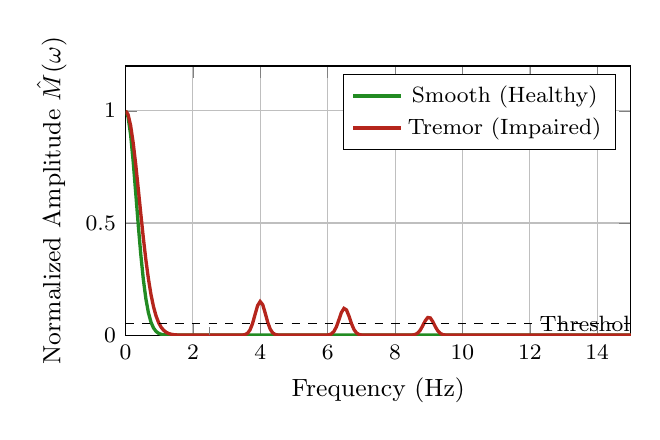
\begin{tikzpicture}
\begin{axis}[
    width=8cm, height=5cm,
    xlabel={Frequency (Hz)},
    ylabel={Normalized Amplitude $\hat{M}(\omega)$},
    xmin=0, xmax=15,
    ymin=0, ymax=1.2,
    grid=major,
    legend pos=north east,
    legend style={font=\footnotesize},
    tick label style={font=\footnotesize},
    label style={font=\small}
]

% Curve A: Smooth / Healthy Movement (single sharp peak, rapid decay)
\addplot[color=ForestGreen, very thick, domain=0:15, samples=200]
    {exp(-5*x^2)};
\addlegendentry{Smooth (Healthy)}

% Curve B: Tremor / Impaired Movement (main peak + harmonic spikes)
\addplot[color=BrickRed, very thick, domain=0:15, samples=200]
    {exp(-3*x^2) + 0.15*exp(-20*(x-4)^2) + 0.12*exp(-20*(x-6.5)^2) + 0.08*exp(-20*(x-9)^2)};
\addlegendentry{Tremor (Impaired)}

% Threshold line (Y = 0.05)
\addplot[color=black, dashed, domain=0:15] {0.05};
\node[anchor=west, font=\footnotesize] at (axis cs:12,0.05) {Threshold};

% Cutoff frequency annotation (vertical line at ω_c ≈ 2.5 Hz for tremor curve)
\draw[gray, dashed] (axis cs:2.5,0) -- (axis cs:2.5,0.05);
\node[anchor=north, font=\footnotesize] at (axis cs:2.5,-0.05) {$\omega_c$};

\end{axis}
\end{tikzpicture}
